\chapter{イジング磁性体から液体--気体臨界現象へ}

\lectureoverview{液体--気体転移には、予想外の道筋から到達できる。まずイジング磁性体の平均場近似による取り扱いを完成させ、その共存線と臨界点を同定し、次に上向きスピンを占有された格子点として読み替える。その結果得られる格子気体は、硬核排除、短距離引力、磁場によって制御される化学ポテンシャルをもち、相図はまったく同じである。形式的な講義は臨界挙動と普遍性で締めくくられる。その後、別個の講義後討論で、物理学者が微調整によって何を意味するのか、選択効果がどのように説明に入り込みうるのか、そしてそのような推論が機構と可能な検証と結びついたときにのみなぜ有用なのかを検討する。}

\section{なぜ沸騰する水は磁石から始まるのか}

沸騰する水は、われわれが理解したい身近な現象である。液体が気体へ変わり、その密度が不連続に変化する。標準的な道筋はファン・デル・ワールス方程式を通る。ここでは別の道筋をとる。イジング磁性体に戻り、その平均場による記述を完成させ、次に同じ模型が流体として読めることを見いだす。

これは単なる絵空事の類推ではない。変数を正しく翻訳してしまえば、イジング磁性体と格子気体は同じ統計力学系である。磁化は粒子密度になり、外部磁場は化学ポテンシャルになり、磁気共存線は液体--気体共存線になる。この翻訳は、見かけ上異なる二つの物質がなぜ同じ臨界挙動をもちうるのかを説明する。

平均場は低次元では厳密な数値解を与えない。一次元では、厳密解が禁じる転移を予言さえする。ここでのその価値は構造的なものである。二次元および三次元では、正しい秩序変数、競合する相、臨界端点、そして無限小のバイアスが一つの相を選び出す仕方を明らかにする。各格子点が六つの最近接格子点をもつ三次元では、それらの隣接格子点をその平均で置き換えるだけでも、すでに有用な定性的描像が得られる。

\section{イジングエネルギー の帳簿付け}

超立方格子上の各格子点に二状態スピンを置く。
\begin{equation}
\sigma_i=\pm1.
\end{equation}
ハミルトニアン
\begin{equation}
\mathcal H
=-J\sum_{\langle ij\rangle}\sigma_i\sigma_j
+h\sum_i\sigma_i,
\qquad J>0.
\label{eq:ising-hamiltonian}
\end{equation}
を用いる。記法が重要である。第一の和は最近接の\emph{リンク}にわたり、第二の和は\emph{格子点}にわたる。リンクは一度だけ数えられ、各端点から一度ずつ数えられるのではない。

単一のリンクに対して、
\begin{equation}
E_{ij}=-J\sigma_i\sigma_j.
\end{equation}
平行スピンはエネルギー\(-J\)をもち、反平行スピンはエネルギー\(+J\)をもつ。したがって、壊れた結合は
\begin{equation}
\Delta E_{\rm bond}=+J-(-J)=2J.
\label{eq:broken-bond}
\end{equation}
のコストを要する。相対的なボルツマン重みを制御するのは、どちらかの絶対的なリンクエネルギーではなく、数\(2J\)である。どの配置にも定数を加えても、いかなる確率も変わらない。

\begin{classroomqa}
\audiencequestion{なぜハミルトニアンには二つの異なる和があるのですか。}
\lecturerresponse{交換エネルギーは隣接する格子点の対に属するので、リンク\(\langle ij\rangle\)にわたって和をとる。場は各スピンに独立に作用するので、格子点\(i\)にわたって和をとる。この二つの数え方を混同すると、まさに平均場で問題になる因子2が導入される。\lecturetimestamp{00:08:04--00:08:45}}
\end{classroomqa}

\begin{classroomqa}
\audiencequestion{\(J\)を大きくすると、単にすべてのエネルギーがより負になるだけですか。}
\lecturerresponse{それは整列した配置と整列していない配置の間の隔たりを大きくする。エネルギーの零点は任意である。物理的な主張は、壊れた結合が\(2J\)のコストを要するということである。したがって、より大きな正の\(J\)は、固定された温度で熱的無秩序をより不利にする。\lecturetimestamp{00:08:47--00:10:17}}
\end{classroomqa}

\(d\)次元の無限または周期的な超立方格子上では、各格子点は\(2d\)個の隣接格子点をもつ。すべての\(N\)個の格子点から数えると各リンクを二度数えるので、
\begin{equation}
N_{\rm links}=\frac{(2d)N}{2}=dN.
\label{eq:number-links}
\end{equation}
したがって、整列した配置は交換エネルギー\(-JdN\)をもつ。境界の格子点は表面項によってこれを変えるが、熱力学極限では\(N\)に比べて無視できる。二つの完全に整列した状態は\(h=0\)のとき縮退している。

場の項は、以後一貫して保つ符号の規約を定める。式~\eqref{eq:ising-hamiltonian}では、正の\(h\)は\(\sigma=-1\)により低い格子点エネルギーを与える。したがって、\(h>0\)は負の磁化を好み、\(h<0\)は正の磁化を好む。\(-h\sum_i\sigma_i\)と書くことによってこの規約を逆にできる。物理的には何も変わらないが、その後のすべての符号はそれに伴って逆にしなければならない。

\begin{classroomqa}
\audiencequestion{ハミルトニアンが\(J\)と\(h\)のみを含むなら、温度はどこから入るのか。}
\lecturerresponse{温度はボルツマン因子\(e^{-\beta\mathcal H}\)を通じて入り、\(\beta=1/T\)は単位\(k_{\rm B}=1\)で測られる。したがって無次元量は\(\beta J\)と\(\beta h\)である。\lecturetimestamp{00:13:07--00:13:43}}
\end{classroomqa}

\section{隣接スピンの平均場の中の一つのスピン}

境界から遠く離れたスピンを選ぶ。それには\(2d\)個の最近接スピンがある。平均場は各々の揺らぐ隣接スピンを同じ平均値で置き換える。
\begin{equation}
m=\expect{\sigma}.
\end{equation}
選んだスピン\(\sigma\)を含む交換エネルギーはそのとき
\begin{equation}
-J\sigma\sum_{\text{\(2d\) neighbors}}\sigma_j
\;\longrightarrow\;-2dJm\,\sigma.
\end{equation}
となる。外部場を加えると、有効一スピンエネルギー
\begin{equation}
\mathcal H_{\rm mf}(\sigma)=(-2dJm+h)\sigma.
\label{eq:mean-field-one-spin}
\end{equation}
が得られる。因子\(2d\)は本質的である。中心スピンの描像を書くときにこれを落としやすく、板書による導出の際に明示的に復元された。

\begin{figure}[ht]
\centering
\includegraphics[width=0.84\textwidth]{lecture_10_figure_02.png}
\caption{平均場の隣接スピンに囲まれた中心スピン、および一スピンエネルギーと発展しつつある自己無撞着方程式。}
\lectureframe{00:17:57}
\end{figure}

一スピン分配関数は
\begin{align}
z_{\rm mf}
&=\sum_{\sigma=\pm1}
\exp\!\left[-\beta(-2dJm+h)\sigma\right] \\
&=2\cosh\!\left[\beta(2dJm-h)\right].
\end{align}
その平均スピンは
\begin{align}
\expect{\sigma}
&=\frac{\sum_{\sigma=\pm1}\sigma
 e^{\beta(2dJm-h)\sigma}}
{\sum_{\sigma=\pm1}e^{\beta(2dJm-h)\sigma}} \\
&=\tanh\!\left[\beta(2dJm-h)\right].
\end{align}
である。しかし選んだスピンは、その平均を\(m\)と呼んだ隣接スピンたちを代表しているはずである。したがって自己無撞着性は
\begin{equation}
\boxed{m=\tanh\!\left[\beta(2dJm-h)\right].}
\label{eq:mean-field-self-consistency}
\end{equation}
を要求する。この一つの非線形方程式が、多スピン問題の平均場による縮約である。

\begin{classroomqa}
\audiencequestion{なぜ左辺の平均は、すべての隣接スピンに対して代入されたのと同じ\(m\)なのか。}
\lecturerresponse{その等式が近似である。一様なバルク状態を仮定し、実際の環境をその平均で置き換え、その環境の中の中心スピンを計算し、計算された平均が仮定した環境を再現することを要求する。解は自己無撞着なバルク状態である。\lecturetimestamp{00:16:28--00:18:00}}
\end{classroomqa}

\begin{equation}
y=2\beta dJm.
\label{eq:y-definition}
\end{equation}
を導入する。\(\beta=1/T\)であるから、
\begin{equation}
m=\frac{yT}{2dJ},
\end{equation}
であり、方程式~\eqref{eq:mean-field-self-consistency}は
\begin{equation}
\boxed{\frac{yT}{2dJ}=\tanh(y-\beta h).}
\label{eq:reduced-mean-field}
\end{equation}
となる。

\begin{figure}[ht]
\centering
\includegraphics[width=0.82\textwidth]{lecture_10_figure_03.png}
\caption{\(y=2\beta dJm\)を導入した後の縮約された自己無撞着方程式。図的に解く準備ができている。}
\lectureframe{00:24:42}
\end{figure}

\begin{classroomqa}
\audiencequestion{なぜ場は\(y-\beta h\)として現れるのか、そして正の場はどのスピンを好むのか。}
\lecturerresponse{我々のハミルトニアンは\(+h\sigma\)を含む。したがってそのボルツマン指数は\(\beta(2dJm-h)\sigma\)であり、双曲線正接は\(y-\beta h\)を含む。正の\(h\)は\(\sigma=-1\)を好む。代わりにハミルトニアンを\(-h\sigma\)で定義すれば、\(h\)の現れる箇所はすべて符号を変え、相図は水平に反転する。\lecturetimestamp{00:18:17--00:20:00}}
\end{classroomqa}

\section{図的解法とキュリー点}

\(h=0\)と置く。我々は
\begin{equation}
\frac{T}{2dJ}y
\qquad\text{and}\qquad
\tanh y.
\end{equation}
の交点を見つけなければならない。第一は原点を通る直線であり、第二は奇関数で飽和する曲線である。高温では直線は急であり、唯一の交点は\(y=0\)、したがって\(m=0\)である。温度が下がるにつれて直線は緩やかになる。臨界温度は、直線と双曲線正接が原点で接するときに達せられる。

\begin{figure}[ht]
\centering
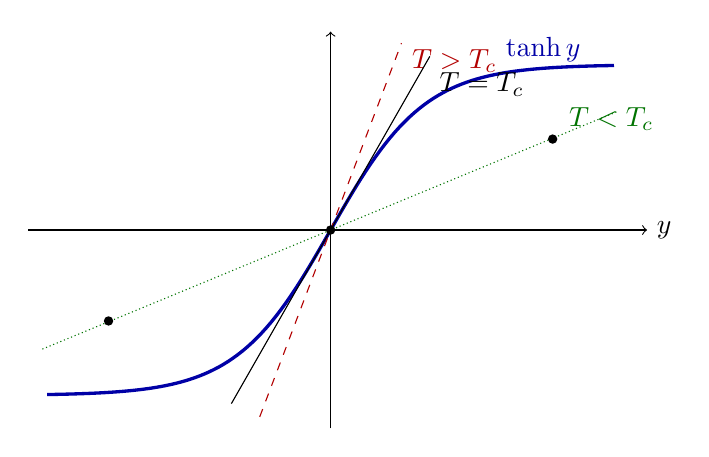
\begin{tikzpicture}[x=1.2cm,y=2.1cm]
\draw[->] (-3.2,0) -- (3.35,0) node[right] {$y$};
\draw[->] (0,-1.2) -- (0,1.2);
\draw[very thick,blue!65!black,domain=-3:3,samples=120]
  plot (\x,{tanh(\x)});
\node[blue!65!black,above] at (2.25,0.96) {$\tanh y$};
\draw[dashed,red!70!black] (-0.75,-1.13) -- (0.75,1.13);
\node[red!70!black,right] at (0.76,1.02) {$T>T_c$};
\draw[black] (-1.05,-1.05) -- (1.05,1.05);
\node[right] at (1.05,0.88) {$T=T_c$};
\draw[densely dotted,green!45!black] (-3.05,-0.72) -- (3.05,0.72);
\node[green!45!black,right] at (2.42,0.67) {$T<T_c$};
\fill (-2.35,-0.55) circle (1.7pt);
\fill (0,0) circle (1.7pt);
\fill (2.35,0.55) circle (1.7pt);
\end{tikzpicture}
\caption{ゼロ場における平均場方程式。\(T_c\)より下では、二つの非零の交点が安定な磁化相を表す。ゼロ解は代数的には依然として存在するが不安定である。}
\label{fig:mean-field-intersections}
\end{figure}

\begin{equation}
\left.\frac{d}{dy}\tanh y\right|_{y=0}=1,
\end{equation}
であるから、接する条件は
\begin{equation}
\frac{T_c}{2dJ}=1.
\end{equation}
である。したがって平均場は
\begin{equation}
\boxed{T_c^{\rm MF}=2dJ.}
\label{eq:sm10-mean-field-tc}
\end{equation}
を予言する。この温度より下では二つの安定な非零解\(\pm m_0(T)\)がある。解\(m=0\)は依然として方程式を満たすが、もはや安定な平衡ではない。系は対称性で結ばれた二つの磁化相の一方を選ぶ。

\begin{classroomqa}
\audiencequestion{これはキュリー温度か。}
\lecturerresponse{はい。強磁性体について、自発磁化が消える温度は慣例的にキュリー温度と呼ばれる。ここで\(2dJ\)はその平均場の値であり、厳密な低次元の結果ではない。\lecturetimestamp{00:28:19--00:28:57}}
\end{classroomqa}

転移の近くで双曲線正接を展開する。
\begin{equation}
\tanh y=y-\frac{y^3}{3}+O(y^5).
\end{equation}
\(h=0\)において、方程式~\eqref{eq:reduced-mean-field}は
\begin{equation}
\left(1-\frac{T}{T_c}\right)y-\frac{y^3}{3}+O(y^5)=0.
\end{equation}
を与える。したがって非零の枝は
\begin{equation}
y^2\simeq3\left(1-\frac{T}{T_c}\right),
\qquad
m\propto(T_c-T)^{1/2}.
\label{eq:mf-beta-exponent}
\end{equation}
のように振る舞う。平方根は平均場の臨界指数である。その正確な値は低次元では生き残らないが、端点における秩序変数の連続的な消失は生き残る。

\section{温度--場平面と枝の選択}

物質は\(J\)を固定する。実験者は\(T\)と\(h\)を変えることができる。したがって\(T\)--\(h\)平面に相図を描くのが自然である。\(T_c\)より下では、任意に小さい場が二つの磁化枝の一方を選ぶ。我々の規約では、\(h<0\)は\(m>0\)を選び、一方\(h>0\)は\(m<0\)を選ぶ。

ゼロ温度ではスピンは完全に揃っているので、\(m=\pm1\) である。高温ではゼロ磁場の平均は \(m=0\) である。\(h=0\) に沿って臨界点に近づくと、大きさ \(m_0(T)\) は連続的にゼロへ減少する。しかし任意の固定した \(T<T_c\) では、\(h=0\) を横切るときに \(+m_0(T)\) から \(-m_0(T)\) へ不連続に切り替わる。

\begin{figure}[ht]
\centering
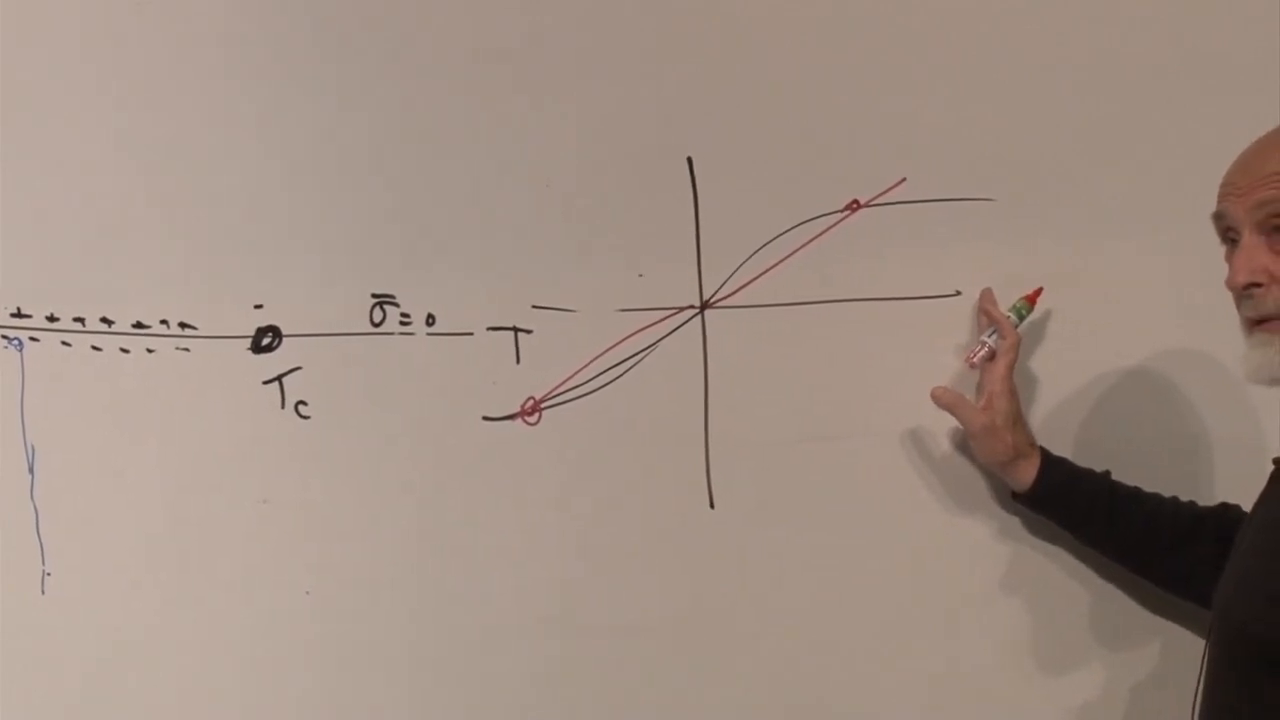
\includegraphics[width=0.90\textwidth]{lecture_10_figure_06.png}
\caption{\(T\)--\(h\) 面における共存線と、\(T_c\) 以下の固定温度における磁化の分枝。}
\lectureframe{00:39:30}
\end{figure}

\begin{figure}[ht]
\centering
\resizebox{\linewidth}{!}{%
\begin{tikzpicture}[x=1.25cm,y=1.15cm]
\begin{scope}
\draw[->] (-2.45,0) -- (2.55,0) node[right] {$h$};
\draw[->] (0,0) -- (0,3.7) node[above] {$T$};
\draw[very thick,red!70!black] (0,0) -- (0,2.35);
\fill[red!70!black] (0,2.35) circle (2.3pt);
\node[right] at (0.08,2.35) {$T_c$};
\node at (-1.25,1.05) {$m>0$};
\node at (1.25,1.05) {$m<0$};
\draw[->,rounded corners,blue!65!black] (-1.65,0.85) -- (-1.65,3.02)
 -- (1.65,3.02) -- (1.65,0.85);
\node[blue!65!black] at (0,3.35) {continuous path};
\end{scope}
\begin{scope}[xshift=7.0cm,yshift=1.55cm]
\draw[->] (-2.5,0) -- (2.5,0) node[right] {$h$};
\draw[->] (0,-1.35) -- (0,1.4) node[above] {$m$};
\draw[very thick,blue!65!black]
  (-2.2,1.05) .. controls (-0.75,1.03) and (-0.2,0.75) .. (-0.08,0.62);
\draw[very thick,blue!65!black]
  (0.08,-0.62) .. controls (0.2,-0.75) and (0.75,-1.03) .. (2.2,-1.05);
\draw[dashed] (0,0.62) -- (0,-0.62);
\fill (0,0.62) circle (1.8pt);
\fill (0,-0.62) circle (1.8pt);
\node at (0,-1.75) {\(T<T_c\)};
\end{scope}
\end{tikzpicture}
}
\caption{固定した \(T<T_c\) では、磁化は共存線を横切って跳ぶ。完全な二パラメータ面では、代わりに臨界点を回り込むことによって二つの相を連続的につなぐことができる。}
\label{fig:ising-phase-plane}
\end{figure}

\begin{classroomqa}
\audiencequestion{\(T_c\) 以下で磁場がちょうどゼロであると何が起こるか。}
\lecturerresponse{理想的な無限系は二つの等しく良好な純粋相をもつ。調製に伴う任意の無限小の残留バイアス、境界条件、または揺らぎが、その一方を選び出す。熱力学的な不連続性は、我々の符号の規約における二つの片側極限 \(m(T,0^-)=+m_0(T)\) と \(m(T,0^+)=-m_0(T)\) によって表される。\lecturetimestamp{00:35:04--00:37:10}}
\end{classroomqa}

\begin{classroomqa}
\audiencequestion{これはヒステリシスと同じことか。}
\lecturerresponse{ヒステリシスは準安定性と、実在系が分枝を切り替える際の履歴に依存した遅れに関わる。それは関連しているが、平衡相図を超えた動力学を必要とし、ここでは展開しない。\lecturetimestamp{00:37:11--00:37:20}}
\end{classroomqa}

\begin{classroomqa}
\audiencequestion{正の相と負の相を不連続性を横切らずにつなぐことができるか。}
\lecturerresponse{できる。温度を \(T_c\) より上に上げ、そこで磁場の符号を変え、再び温度を下げる。その経路は端点を回り込み、磁化は連続的に変化する。跳びが避けられないのは、固定した \(T<T_c\) で \(h=0\) を横切るときだけである。\lecturetimestamp{00:37:20--00:38:15}}
\end{classroomqa}

\begin{classroomqa}
\audiencequestion{\(h\) がゼロに近づくときはいつでも磁化はゼロに近づくか。}
\lecturerresponse{\(T_c\) 以下の一般的な温度ではそうではない。そこでは片側極限は非ゼロである。自発磁化がゼロに近づくのは、臨界温度そのものに近づくときだけである。\lecturetimestamp{00:38:29--00:39:45}}
\end{classroomqa}

\section{透過性の箱と化学ポテンシャル}

ここで磁石を離れ、再び粒子から始める。周囲の空間よりポテンシャルエネルギーが低い領域を想像しよう。壁は透過性である。すなわち粒子は出入りできる。内部のエネルギーが量 \(\mu\) だけ低いなら、内部の占有は相対的なボルツマン因子 \(e^{\beta\mu}\) を受け取る。井戸を深くしたり浅くしたりすると、箱の中の平均粒子数が変わる。

\begin{figure}[ht]
\centering
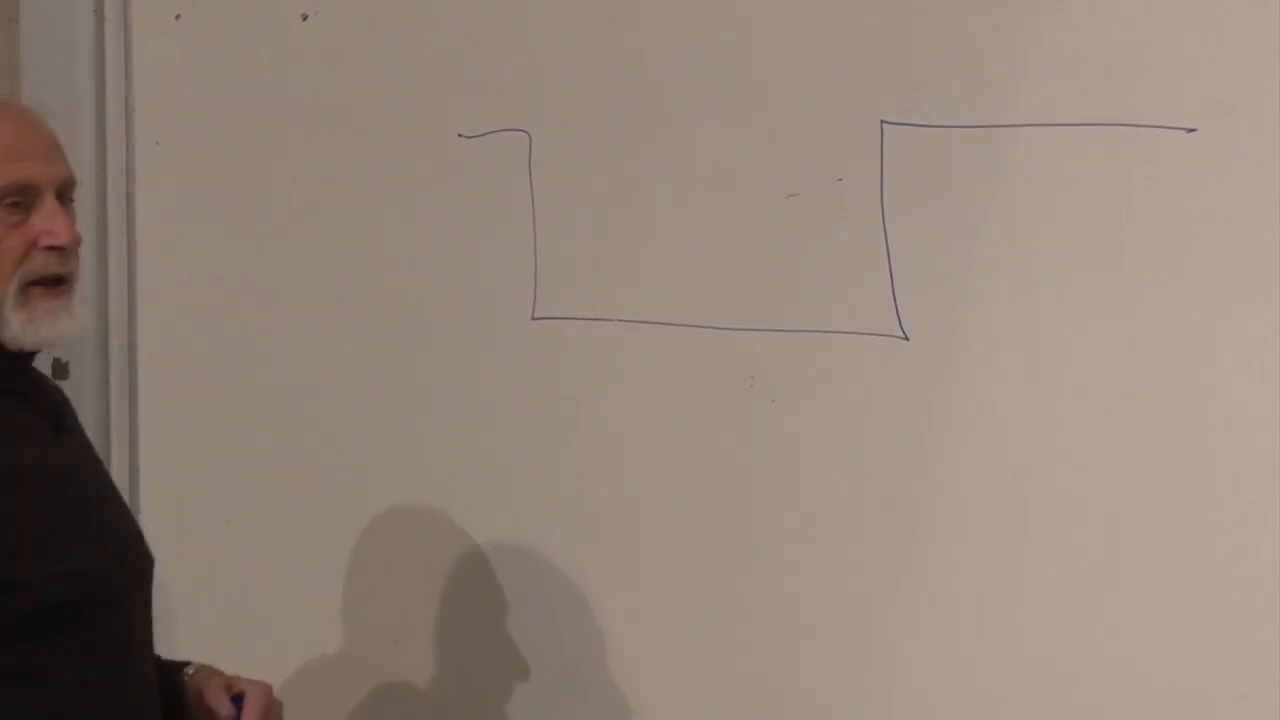
\includegraphics[width=0.84\textwidth]{lecture_10_figure_07.png}
\caption{透過性の箱のポテンシャル井戸の描像。内部と外部のエネルギー差が、粒子が箱を占める選好を制御する。}
\lectureframe{00:41:30}
\end{figure}

\begin{figure}[ht]
\centering
\resizebox{\linewidth}{!}{%
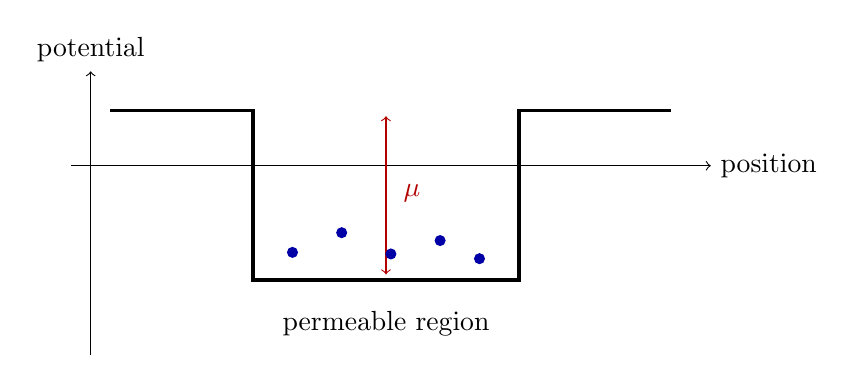
\begin{tikzpicture}[x=1.25cm,y=1.0cm]
\draw[->] (-3.2,0) -- (3.3,0) node[right] {position};
\draw[->] (-3.0,-2.4) -- (-3.0,1.2) node[above] {potential};
\draw[very thick] (-2.8,0.7) -- (-1.35,0.7)
 -- (-1.35,-1.45) -- (1.35,-1.45) -- (1.35,0.7) -- (2.9,0.7);
\draw[<->,red!70!black] (0,0.63) -- (0,-1.38);
\node[right,red!70!black] at (0.08,-0.35) {$\mu$};
\foreach \x/\y in {-0.95/-1.1,-0.45/-0.85,0.05/-1.12,0.55/-0.95,0.95/-1.18}
  \fill[blue!65!black] (\x,\y) circle (2pt);
\node at (0,-2.0) {permeable region};
\end{tikzpicture}
}
\caption{ポテンシャルのオフセットを変えると粒子数の選好が変わる。大正準記述では、そのオフセットは化学ポテンシャルによって表される。}
\end{figure}

この思考実験は化学ポテンシャルを具体的にする。それは貯蔵庫に対して加えられた粒子一つあたりのエネルギー上の利得である。複数の種が壁を通り抜けられるなら、各々の種がそれ自身の化学ポテンシャルをもつ。密閉された箱は異なる。その場合 \(N\) は固定され、化学ポテンシャルは貯蔵庫との交換によって課されるのではなく、熱力学的に推論される。

\begin{classroomqa}
\audiencequestion{井戸の深さは文字通り化学ポテンシャルか。}
\lecturerresponse{それは化学ポテンシャル差の直接的な力学的実現である。内部のすべての一粒子準位を \(\mu\) だけ下げることは、エネルギーに \(-\mu N\) を寄与し、したがってボルツマン指数に \(+\beta\mu N\) を寄与する。化学ポテンシャルの差だけが意味をもつ。\lecturetimestamp{00:44:49--00:45:40}}
\end{classroomqa}

粒子が出入りできるので、分配和はすべての粒子数を含まなければならない。
\begin{equation}
\Xi(T,\mu)
=\sum_{N=0}^{\infty}\;\sum_{\mathcal C_N}
\exp\!\left[-\beta E(\mathcal C_N)+\beta\mu N\right].
\label{eq:grand-partition}
\end{equation}
内側の和は指定された \(N\) をもつ配置にわたって走り、外側の和は \(N\) そのものにわたって走る。大正準重みは \(e^{-\beta(E-\mu N)}\) とも書ける。

\begin{figure}[ht]
\centering
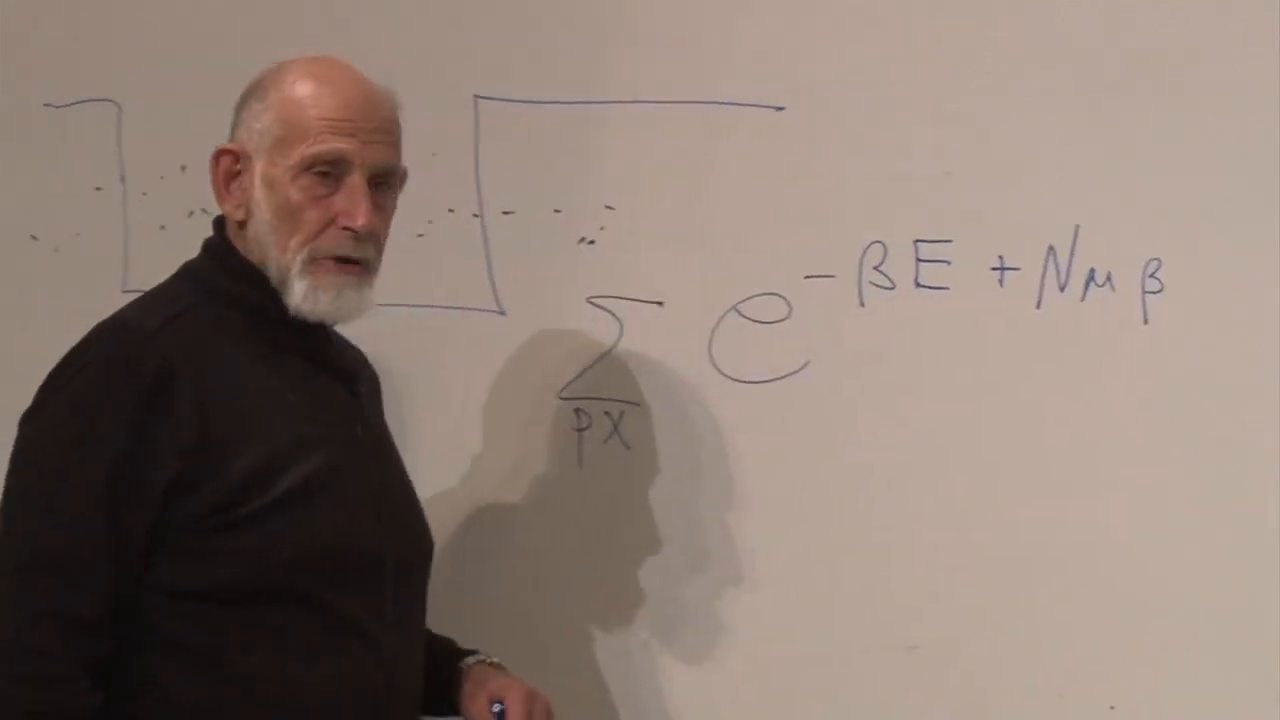
\includegraphics[width=0.88\textwidth]{lecture_10_figure_08.png}
\caption{透過性の箱と、粒子数および配置にわたる大正準和。}
\lectureframe{00:47:15}
\end{figure}

\begin{classroomqa}
\audiencequestion{箱が密閉されると何が変わるか。}
\lecturerresponse{粒子数は揺らがなくなる。そのとき固定した \(N\) における正準分配関数を用いる。透過性の箱では、\(N\) は \(\mu\) によって平均的に制御される熱力学変数である。\lecturetimestamp{00:45:42--00:47:50}}
\end{classroomqa}

一定温度では、\(\mu\)を変えると通常は密度が滑らかに変化する。臨界温度以下では、代わりに不連続な跳びを引き起こすことがある。それこそが我々の求めている流体現象である。これを微視的に得るには、粒子に二つの特徴が必要である。すなわち、同じ場所を占めることができてはならず、短距離で引き合わなければならない。

\section{スピンを格子気体に変える}

格子はそのままにして、その二つの状態を読み替える。占有数
\begin{equation}
n_i=\frac{1+\sigma_i}{2}
=
\begin{cases}
0,&\sigma_i=-1,\\
1,&\sigma_i=+1.
\end{cases}
\label{eq:occupation-map}
\end{equation}
を定義する。空のサイトはスピン下向き、占有されたサイトはスピン上向きである。\(n_i\)は0か1しかとれないので、二重占有は禁止される。したがって格子自体が剛体芯を与える。

\begin{figure}[ht]
\centering
\includegraphics[width=0.84\textwidth]{lecture_10_figure_04.png}
\caption{格子気体との対応付けは、\(\sigma=-1\)を空のサイトとすることから始まる。すると\(\sigma=+1\)は占有されたサイトである。}
\lectureframe{00:53:45}
\end{figure}

空の格子、すなわちすべて\(\sigma=-1\)から始める。すべての結合は揃っており、エネルギー\(-J\)をもつ。この一定の真空エネルギーは差し引くことができる。次に2次元で1個の粒子をサイトに置く。対応するスピンは\(+1\)に反転し、4本の結合を壊す。壊れた結合はそれぞれ\(2J\)のコストがかかるので、
\begin{equation}
\Delta E_1=4(2J)=8J.
\label{eq:one-particle-cost}
\end{equation}
遠く離れた2個の粒子は8本の結合を壊し、\(16J\)のコストがかかる。2個の粒子が隣接するサイトを占めるなら、それらの間の結合は再び揃う。壊れる境界結合は6本だけであり、コストは
\begin{equation}
\Delta E_{2,\rm adjacent}=6(2J)=12J.
\end{equation}
したがって粒子を近づけるとエネルギーが
\begin{equation}
16J-12J=4J.
\label{eq:lattice-attraction}
\end{equation}
だけ下がる。この生の数え上げは最初\(2J\)の節約として述べられ、その後訂正された。共有された1本の結合が壊れた境界への寄与を二つ取り除くので、引力は\(4J\)である。

\begin{figure}[ht]
\centering
\includegraphics[width=0.84\textwidth]{lecture_10_figure_05.png}
\caption{2次元の結合の数え上げ：孤立した1個の粒子は\(8J\)、遠く離れた2個の粒子は\(16J\)、隣接する2個の粒子は\(12J\)のコストがかかる。}
\lectureframe{01:00:25}
\end{figure}

格子気体は今や必要な分子論的性質を両方備えている。二値的な占有が剛体芯排除を与え、交換相互作用が強さ\(4J\)の最近接引力を与える。スピン反転が占有サイトの数を変えるので、粒子数は揺らぐことが許される。

\subsection{厳密な代数的対応辞書}

結合を数える描像で物理を見るには十分だが、変数変換を正確に行えば等価性は紛れもなくなる。
\begin{equation}
\sigma_i=2n_i-1
\end{equation}
を式~\eqref{eq:ising-hamiltonian}に代入する。リンクについて、
\begin{equation}
\sigma_i\sigma_j
=4n_in_j-2n_i-2n_j+1.
\end{equation}
正則な\(d\)次元格子では、
\begin{equation}
\sum_{\langle ij\rangle}(n_i+n_j)=2d\sum_i n_i.
\end{equation}
したがって
\begin{align}
\mathcal H
&=-4J\sum_{\langle ij\rangle}n_in_j
+(4dJ+2h)\sum_i n_i+\text{constant}.
\label{eq:ising-as-lattice-gas}
\end{align}
これを従来の格子気体ハミルトニアン
\begin{equation}
\mathcal H_{\rm lg}
=-\epsilon\sum_{\langle ij\rangle}n_in_j
-\mu\sum_i n_i+\text{constant}.
\label{eq:lattice-gas-hamiltonian}
\end{equation}
と比較する。対応関係は
\begin{equation}
\boxed{\epsilon=4J,\qquad
\mu=-(4dJ+2h).}
\label{eq:chemical-potential-map}
\end{equation}

\begin{figure}[ht]
\centering
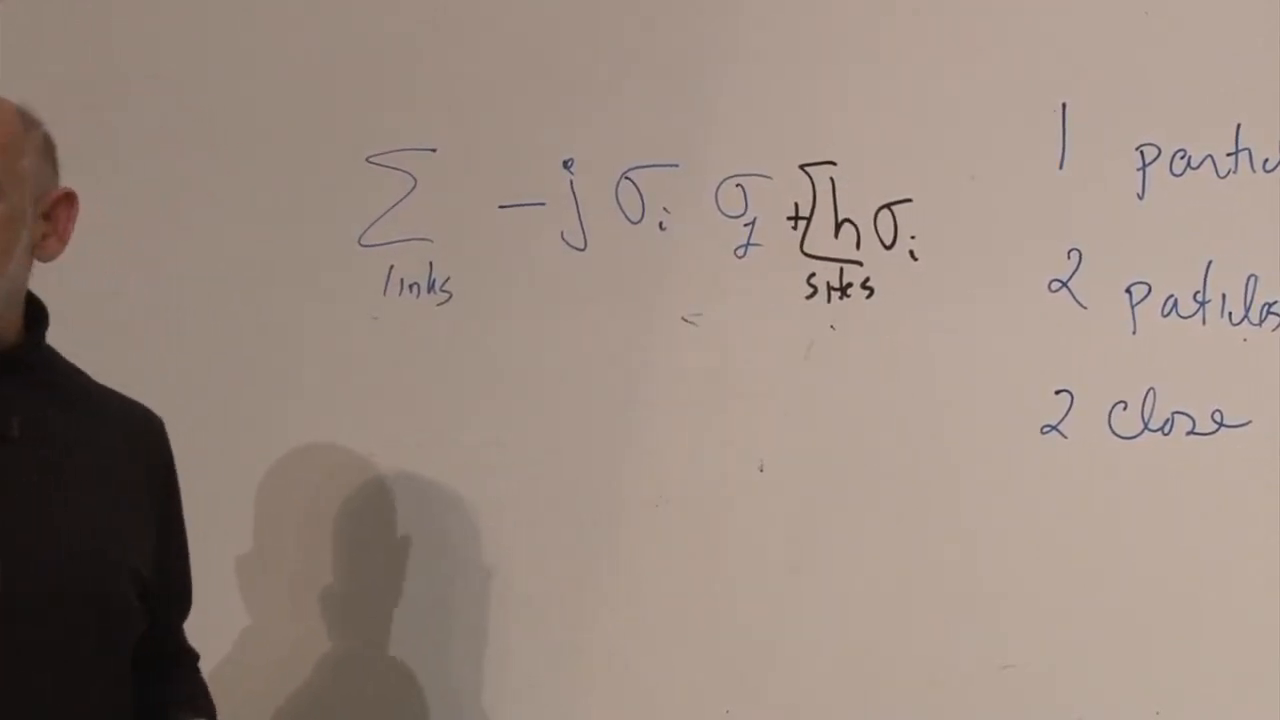
\includegraphics[width=0.88\textwidth]{lecture_10_figure_09.png}
\caption{粒子エネルギーの数え上げの隣に並べた交換項と場の項。場は最近接引力を変えずに挿入エネルギーを変える。}
\lectureframe{01:04:30}
\end{figure}

2次元では、孤立した挿入はエネルギーを
\begin{equation}
8J+2h=-\mu.
\end{equation}
だけ変える。\(8J\)は壊れた結合から来ており、\(2h\)は1個のスピンを\(-1\)から\(+1\)へ変えることから来る。したがって\(h\)を調整すると、引力\(4J\)を固定したまま化学ポテンシャルを調整することになる。場は文字通り\(\mu\)に等しいわけではない。交換の基準値がオフセット\(4dJ\)に寄与するからである。

\begin{classroomqa}
\audiencequestion{場が粒子数を制御するなら、なぜ\(h\)は単に化学ポテンシャルではないのか。}
\lecturerresponse{粒子を生成することは、空の参照状態に対して交換結合も壊す。したがって\(-N\)の従来の係数は\(\mu=-(4dJ+2h)\)であり、単に\(-2h\)ではない。オフセットは\(J\)と配位数に依存する。\lecturetimestamp{01:06:28--01:06:41}}
\end{classroomqa}

密度も同様に単純である。
\begin{equation}
\rho=\expect{n_i}
=\frac{1+\expect{\sigma_i}}{2}
=\frac{1+m}{2}.
\label{eq:density-map}
\end{equation}
したがって\(m=-1\)は空の格子、\(m=+1\)は完全に満たされた格子、\(m=0\)は半充填である。全粒子数は\(N_{\rm p}=\sum_i n_i\)であり、密度は\(N_{\rm p}/N\)である。

\begin{figure}[ht]
\centering
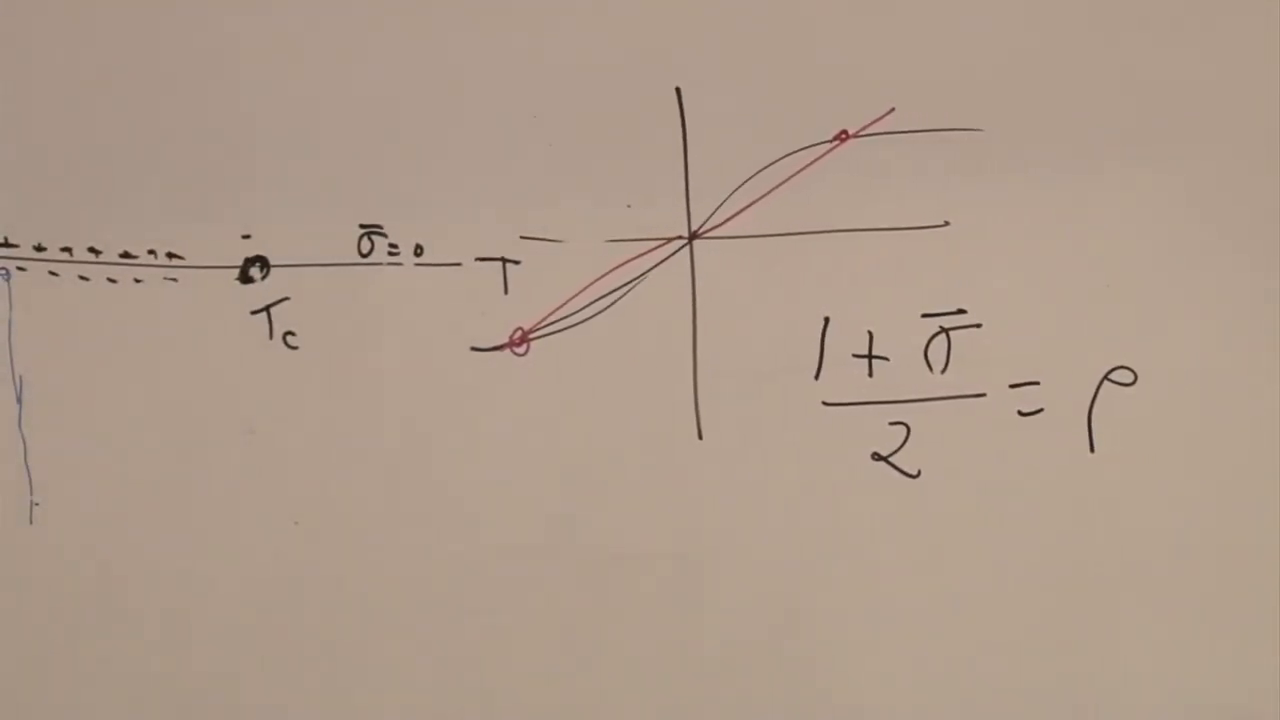
\includegraphics[width=0.90\textwidth]{lecture_10_figure_10.png}
\caption{磁気共存線の隣に書かれた密度関係\(\rho=(1+m)/2\)。}
\lectureframe{01:08:25}
\end{figure}

\begin{classroomqa}
\audiencequestion{\((1+m)/2\)は粒子数か、それとも密度か。}
\lecturerresponse{それはサイトあたりの平均占有数であり、したがって無次元の格子密度である。全サイト数を掛けると期待粒子数が得られる。示強的な密度と示量的な数え上げの区別は重要である。\lecturetimestamp{01:06:43--01:09:31}}
\end{classroomqa}

\section{磁気相図が流体相図になる}

式~\eqref{eq:chemical-potential-map}と\eqref{eq:density-map}を用いて図~\ref{fig:ising-phase-plane}を読み替える。\(T_c\)より上では、\(\mu\)を変えると密度が滑らかに変化する。\(T_c\)より下では、共存値
\begin{equation}
\mu_{\rm coex}=-4dJ
\qquad(h=0)
\label{eq:coexistence-mu}
\end{equation}
を横切ると密度が希薄気体と高密度液体の間で跳ぶ。\(T_c\)では二つの密度が合流し、不連続性が消える。

\begin{figure}[ht]
\centering
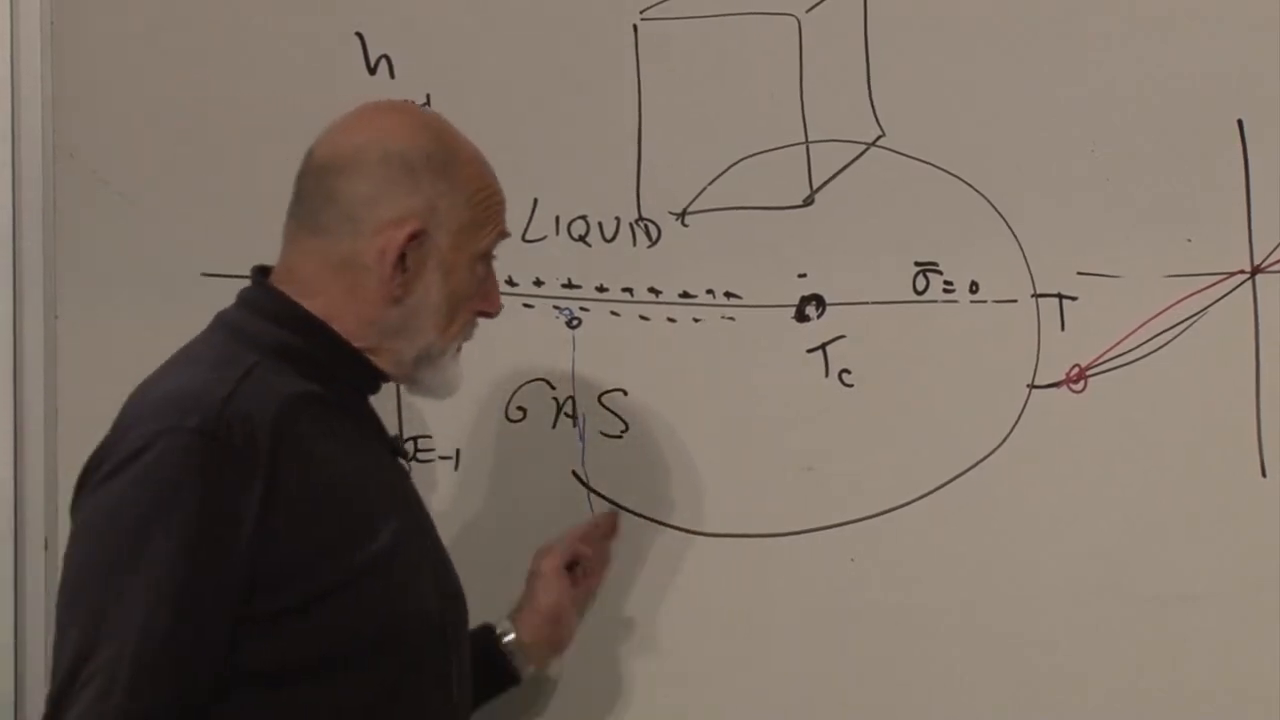
\includegraphics[width=0.92\textwidth]{lecture_10_figure_11.png}
\caption{Isingの共存線を液体--気体の相図として読む。気体は低密度側に、液体は高密度側にあり、両者は臨界端点の周りを連続的につなぐことができる。}
\lectureframe{01:14:30}
\end{figure}

\begin{figure}[ht]
\centering
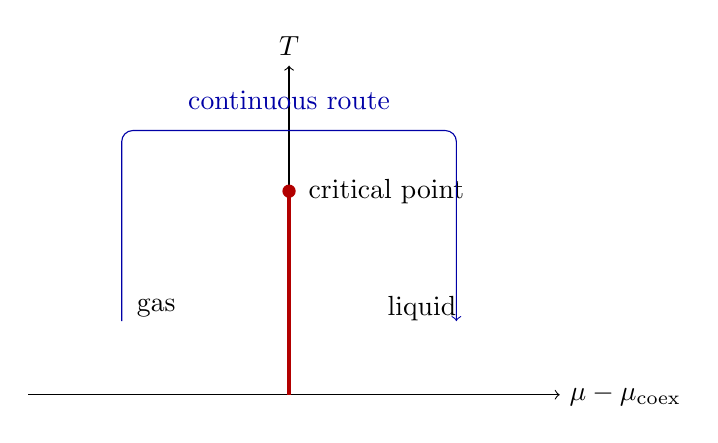
\begin{tikzpicture}[x=1.25cm,y=1.1cm]
\draw[->] (-2.65,0) -- (2.75,0) node[right] {$\mu-\mu_{\rm coex}$};
\draw[->] (0,0) -- (0,3.8) node[above] {$T$};
\draw[very thick,red!70!black] (0,0) -- (0,2.35);
\fill[red!70!black] (0,2.35) circle (2.4pt);
\node[right] at (0.1,2.35) {critical point};
\node at (-1.35,1.0) {gas};
\node at (1.35,1.0) {liquid};
\draw[->,blue!65!black,rounded corners]
 (-1.7,0.85) -- (-1.7,3.05) -- (1.7,3.05) -- (1.7,0.85);
\node[blue!65!black] at (0,3.4) {continuous route};
\end{tikzpicture}
\caption{端点より下では液体と気体は別個の相であるが、超臨界領域ではそれらを隔てる特異な境界は存在しない。}
\label{fig:liquid-gas-plane}
\end{figure}

これはよく知られた沸騰線を同定する。一定の圧力のもとで液体を加熱し共存線を越えると沸騰が起こる。一定の温度のもとでは、圧力または化学ポテンシャルを変えることによって同じ境界を越えることができる。過熱蒸気や過冷却液体は平衡共存を越えた準安定な継続であり、その寿命を記述するには核生成の動力学が必要であって、それはこの平衡論的な構成の範囲を超えている。

\begin{classroomqa}
\audiencequestion{過熱蒸気はこの相図に表されているか。}
\lecturerresponse{平衡相図は共存境界を同定する。過熱状態または過飽和状態は準安定である。すなわち、臨界液滴を形成するには界面自由エネルギーのコストがかかるため、誤った側に一時的にとどまる。この動力学による精密化はここでは計算しない。\lecturetimestamp{01:12:19--01:12:29}}
\end{classroomqa}

\begin{classroomqa}
\audiencequestion{通常の流体では化学ポテンシャルをどのように変えるのか。}
\lecturerresponse{ポテンシャル井戸の箱が理論的に最も明快な制御である。実験室では圧力、体積、またはリザーバーとの接触を変えることのほうが多く、熱力学がそれらの制御を化学ポテンシャルの変化へと翻訳する。\lecturetimestamp{01:12:30--01:13:59}}
\end{classroomqa}

\begin{classroomqa}
\audiencequestion{密度が変化するとき、分子ポテンシャル\(J\)を変えているのか。}
\lecturerresponse{いいえ。固定された物質に対して、\(J\)は短距離引力を表し、この模型では固定されている。\(\mu\)を変えると、いくつのサイトが占有されるかが変わり、したがって分子間距離の分布が変わる。\(J\)を変えることは、微視的な物質または相互作用を変えることを意味する。\lecturetimestamp{01:14:50--01:15:41}}
\end{classroomqa}

\begin{classroomqa}
\audiencequestion{臨界温度は通常の沸点と同じものか。}
\lecturerresponse{いいえ。沸点は選ばれた圧力のもとで指定されるので、圧力が変われば共存曲線に沿って移動する。臨界温度は、それを超えると液体と気体がもはや相境界によって隔てられなくなる唯一の端点である。この格子気体の扱いでは圧力は陽に導出されていない。\lecturetimestamp{01:15:42--01:17:02}}
\end{classroomqa}

ここで中心的な結果を述べることができる。Ising磁性体と格子気体は単に似た図を描くだけではない。変数とパラメータの変換の後、それらは分配関数を共有する。一方の側のすべての特異な熱力学的性質は、他方の側に対応するものをもつ。
\begin{equation}
\begin{array}{c|c}
\text{Ising magnet} & \text{lattice gas}\\ \hline
\sigma_i=\pm1 & n_i=0,1\\
m=\expect{\sigma} & \rho=(1+m)/2\\
h & \mu=-(4dJ+2h)\\
\text{aligned exchange} & \text{nearest-neighbor attraction}\\
h=0,\ T<T_c & \text{liquid--gas coexistence}\\
(T_c,0) & \text{critical endpoint}
\end{array}
\label{eq:ising-fluid-dictionary}
\end{equation}

\section{臨界指数と普遍性}

臨界点の近くでは、熱力学的量はしばしば冪則的な特異性を示す。換算温度
\begin{equation}
t=\frac{T-T_c}{T_c},
\end{equation}
を用いて、模式的には次のように書ける。
\begin{equation}
m\sim(-t)^{\beta_{\rm crit}},
\qquad
\chi\sim |t|^{-\gamma},
\qquad
\xi\sim |t|^{-\nu}.
\label{eq:critical-exponents}
\end{equation}
ここで\(\beta_{\rm crit}\)は臨界指数であり、逆温度ではない。平均場では\(\beta_{\rm crit}=1/2\)を与えるが、揺らぎは上限臨界次元より下で指数を変える。

指数は整数である必要はない。またすべてが無理数である必要もない。二次元Ising模型は有名なことにいくつかの厳密な有理指数をもつ一方、三次元Isingの値は理論と計算によって高い精度で決定された非自明な数である。頑健な教訓は、指数は一般に初等的な次元解析によって固定されるものではないということである。

さらに驚くべきことに、微視的な詳細がそれらを固定しないことが多い。同じ空間次元、同じ秩序変数の対称性、そして十分に短距離の相互作用をもつ系は、同じ長距離臨界理論へと流れることができる。それらは一つの\emph{普遍性クラス}に属する。一軸磁性体と通常の液体--気体端点はどちらも単一のスカラー秩序変数をもち、同じ次元のIsing普遍性クラスを共有する。

\begin{classroomqa}
\audiencequestion{普遍性クラスは有限または離散的なリストなのか。}
\lecturerresponse{多くのクラスがあり、次元、対称性、保存則、相互作用の到達距離、その他の長距離的データによって組織される。多くのよく知られた場合では固定点と指数の組は離散的であるが、指数が連続的に変化する系も存在する。安全な主張は、目録が有限であるということではなく、多くの微視的に異なる系が同じ長距離的データを共有するということである。\lecturetimestamp{01:18:50--01:19:38}}
\end{classroomqa}

\begin{classroomqa}
\audiencequestion{液体と気体が共存するとき、実際の容器の中で両者を隔てているものは何か。}
\lecturerresponse{界面である。表面張力は界面の面積にペナルティを与え、重力は鉛直方向の化学ポテンシャル勾配を生み出し、通常はより密度の大きい液体を気体の下に置く。無視できる重力のもとでは、幾何学的配置は表面張力と境界条件によってより直接的に支配される。\lecturetimestamp{01:19:40--01:21:18}}
\end{classroomqa}

\begin{classroomqa}
\audiencequestion{この描像において気化熱はどこにあるのか。}
\lecturerresponse{臨界点より下では、一次相転移の共存線を横切ることは一般に潜熱を伴う。二つの相がそこで同一になるため、臨界端点に近づくにつれて気化熱はゼロに近づく。この講義は相構造を確立するが、潜熱を計算するものではない。\lecturetimestamp{01:21:19--01:22:18}}
\end{classroomqa}

\begin{classroomqa}
\audiencequestion{相転移を、例えば超伝導デバイスを用いて、敏感な検出器として使うことができるか。}
\lecturerresponse{できる。転移の近くでは、小さな摂動が大きな応答を生み出したり、状態の変化を引き起こしたりしうる。実用的な検出器はその感度を利用するが、関係する秩序変数やダイナミクスはイジングの例とは異なるかもしれない。\lecturetimestamp{01:22:19--01:24:05}}
\end{classroomqa}

これで統計力学の講義を終える。その道筋はエントロピーと平衡から始まり、分配関数と気体を経て、磁石と流体が同一の臨界現象の二つの記述でありうることを示して終わる。

\section{講義後の議論：微調整と選択}

正式な講義が終わった後、会話はおよそ四十分にわたって続いた。それは記録に残す価値があるが、上記の導出と混同されるべきではない。主題はもはや格子気体ではない。それは微調整の論理と、宇宙論における人間原理的選択の慎重な使用である。

\subsection{小さな数は自動的に微調整されているわけではない}

\emph{人間原理}という語句のあらゆる用法を決着させる単一の文は存在しない。有用な出発点は操作的である。すなわち、ある理論が多数の実現された環境を許すとき、観測は、観測者が生じうるのはそれらの一部においてのみであるという事実に条件づけられる。その条件付きの言明は合理的でありうる。しかし、アンサンブル、選択条件、あるいは代替案を物理的に意味あるものにする機構を伴わずに持ち出されるならば、それは空虚になる。

選択が入り込む前に、小さなパラメータと微調整されたパラメータとを区別しなければならない。ある数が小さいのは、安定な力学的機構がそれを特別な値へと駆動するからでありうる。微調整とは、観測された値が、それ以外では独立な寄与の間の並外れて精密な釣り合いを要求しているように見え、その釣り合いを保護する既知の復元機構も対称性も存在しないことを意味する。

\begin{classroomqa}
\audiencequestion{人間原理は鋭く述べることができるか。}
\lecturerresponse{その擁護可能な用法は、神秘的というよりも条件付きである。すなわち、多数の物理的に実現された環境が異なるパラメータをもつならば、我々のような存在によって観測される環境は、観測者と両立する部分集合から引き出される。そのこと自体は環境を生成したり、それらの確率を割り当てたりするものではない。それらの課題は根底にある物理学に属する。\lecturetimestamp{01:25:45--01:26:13}}
\end{classroomqa}

宇宙定数はその動機となる例である。その観測された大きさは、真空エネルギーへの素朴な量子場理論的寄与と比べて並外れて小さい。困難は、単に最終的な数が小さいことではない。多くの大きな項が途方もない精度で相殺しなければならないように見える一方で、結果を観測値へと調整する、受け入れられた低エネルギー・フィードバック機構が存在しないことである。

\subsection{飛行船と潜水艦}

二つの浮力の例がこの区別を際立たせる。飛行船は、その平均密度が周囲の空気の密度と一致する高度に浮かぶ。空気の密度は高度とともに減少する。飛行船が上昇すれば、外部の空気はより希薄になり、飛行船は下降しようとする。下降すれば、外部の空気はより密になり、飛行船は上昇しようとする。密度の一致は数値的に微妙でありうるが、大気の勾配が復元フィードバックを与える。この平衡は力学的に説明される。

ほぼ非圧縮性の水中で中性浮力をとる潜水艦は異なる。水の密度は深さによってほとんど変化しない。潜水艦の平均密度がたまたま周囲の水と等しくなったとしても、その等しさを説明する、深さに依存する同程度の復元機構は存在しない。わずかな不一致が潜水艦を上昇させたり沈めたりする。中性浮力を達成するには、バラストと内容物の精密な調整が必要である。そのとき、何らかの制御系や設計機構がそれを説明しない限り、小さな残差は微調整である。

\begin{figure}[ht]
\centering
\resizebox{\linewidth}{!}{%
\begin{tikzpicture}[>=Latex]
\begin{scope}[xshift=-3.8cm]
\shade[top color=blue!5,bottom color=blue!28] (-2.5,-2.2) rectangle (2.5,2.2);
\draw[very thick,rounded corners=18pt,fill=yellow!35]
  (-1.15,0) ellipse (1.15 and 0.55);
\draw[thick] (0,-0.55) -- (0,-1.05);
\draw[thick,fill=gray!20] (-0.45,-1.05) rectangle (0.45,-1.38);
\draw[->,red!70!black,thick] (1.65,1.45) -- (1.65,0.55)
 node[midway,right] {restoring};
\draw[->,red!70!black,thick] (-1.65,-1.45) -- (-1.65,-0.55)
 node[midway,left] {restoring};
\node at (0,2.55) {\textbf{Blimp: density gradient}};
\node[align=center] at (0,-2.75) {displacement changes\\the buoyant imbalance};
\end{scope}
\begin{scope}[xshift=3.8cm]
\shade[top color=cyan!10,bottom color=blue!45] (-2.5,-2.2) rectangle (2.5,2.2);
\draw[very thick,fill=gray!35,rounded corners=12pt]
  (-1.45,-0.25) -- (1.1,-0.25) arc (-90:90:0.38)
  -- (-1.45,0.51) -- cycle;
\draw[thick] (-0.25,0.51) -- (-0.25,0.85) -- (0.35,0.85) -- (0.35,0.51);
\draw[->,red!70!black,thick] (1.65,0.15) -- (1.65,1.35)
 node[midway,right] {rise};
\draw[->,red!70!black,thick] (-1.65,0.15) -- (-1.65,-1.35)
 node[midway,left] {sink};
\node at (0,2.55) {\textbf{Submarine: nearly uniform density}};
\node[align=center] at (0,-2.75) {no depth-dependent feedback\\protects neutral buoyancy};
\end{scope}
\end{tikzpicture}
}
\caption{小さな残差は、力学的に安定でありうるし、真に調整されたものでもありうる。飛行船には復元フィードバックがあるが、理想化された潜水艦では、その平均密度を水に合わせて調整する必要がある。}
\label{fig:blimp-submarine}
\end{figure}

\begin{classroomqa}
\audiencequestion{中性浮力が観測されたなら、なぜ潜水艦の乗員は説明を要求すべきなのか。}
\lecturerresponse{バラスト制御機構がなければ、対称性も環境フィードバックも、二つの独立な密度の等しさを保護しないからである。問題は、その等しさが論理的に可能かどうかではなく、なぜ系がそのパラメータ空間のごく狭い領域を占めるのかである。\lecturetimestamp{01:35:05--01:36:25}}
\end{classroomqa}

\subsection{多数の領域と条件付き観測}

ここで、多くの異なる平均密度をもつ膨大な数の潜水艦を生成する過程を想像しよう。大半は沈むか浮き上がり、ごく一部だけが水面と海底の間の居住可能帯にとどまる。必然的に生き残った潜水艦の一つに住む観測者は、ほぼ中性の浮力を測定しても驚くべきではない。その観測は、観測者が存在するために必要な条件によって選択されている。

この推論には二つの要素が必要である。
\begin{enumerate}
\item 想像の中にのみ存在する代替案ではなく、実際に多くの代替案を実現する物理的過程。
\item なぜ観測が制限された部分集合においてのみなされるのかを説明する選択条件。
\end{enumerate}
選択は生成機構を置き換えるものではない。それは、アンサンブルが存在したときに観測者が何を測定するかの条件付き確率を変える。

\begin{classroomqa}
\audiencequestion{この議論は、十分に大きな標本のどこかで起こる unlikely な事柄にすぎないというものか。}
\lecturerresponse{それは前半にすぎない。後半は観測的条件付けである。観測者はすべての領域から一様に抽出されるのではなく、その存在が可能な領域からのみ抽出される。完全な提案には依然として、領域上の測度と、それらがどのように生成されるかの物理的説明が必要である。\lecturetimestamp{01:39:19--01:40:36}}
\end{classroomqa}

真空エネルギーに適用すると、大きな負の宇宙定数は宇宙を急速に再収縮させうるが、十分に大きな正の値は物質が銀河へ凝縮するのを妨げうる。観測値は、長寿命の構造と両立する狭い範囲にある。これは可能な選択条件を与えるが、宇宙定数の分布の導出ではない。

量子場の理論は微調整問題を付け加える。異なる場とスケールからの真空寄与は、それぞれが観測された残差よりはるかに大きい。それらの項がほぼ正確に相殺するなら、結果は自己修正する飛行船というより、注意深く釣り合わされた潜水艦に似る。この類推は論理的問題を明らかにするためのものであり、その解決を与えるためのものではない。

\begin{classroomqa}
\audiencequestion{一つのパラメータの変化を、他のいくつかのパラメータの変化で補償できるか。}
\lecturerresponse{できる。生存可能な集合は一つの軸上の狭い区間である必要はなく、多次元パラメータ空間内の薄い面でありうる。相関した変化は構造を保ちうるが、そのとき問題は、なぜ実現したパラメータがその面の近くにあるのか、また基礎理論がそれにどのような測度を割り当てるのかである。\lecturetimestamp{01:45:10--01:46:19}}
\end{classroomqa}

\begin{figure}[ht]
\centering
\begin{tikzpicture}[x=1.3cm,y=1.05cm,>=Latex]
\draw[->] (-3.2,0) -- (3.4,0) node[right] {$\lambda_1$};
\draw[->] (0,-2.5) -- (0,2.65) node[above] {$\lambda_2$};
\fill[gray!12] (-3,-2.25) rectangle (3.1,2.3);
\draw[very thick,blue!65!black]
 (-2.8,-1.55) .. controls (-1.3,-0.75) and (0.15,0.05) .. (2.85,1.55);
\draw[very thick,blue!25]
 (-2.8,-1.25) .. controls (-1.3,-0.45) and (0.15,0.35) .. (2.85,1.85);
\fill[blue!15,opacity=.65]
 (-2.8,-1.55) .. controls (-1.3,-0.75) and (0.15,0.05) .. (2.85,1.55)
 -- (2.85,1.85) .. controls (0.15,0.35) and (-1.3,-0.45) .. (-2.8,-1.25) -- cycle;
\node[blue!65!black,rotate=28] at (1.3,0.95) {viable band};
\foreach \x/\y in {-2.4/1.45,-1.7/-1.8,-0.9/1.8,0.3/-1.45,1.2/1.85,2.4/-0.8}
  \fill[red!65!black] (\x,\y) circle (2pt);
\fill[green!45!black] (0.55,0.58) circle (2.8pt);
\node[green!35!black,right] at (0.65,0.55) {observed domain};
\end{tikzpicture}
\caption{複数のパラメータがある場合、居住可能性や構造的生存可能性は、一つのパラメータの狭い区間ではなく、薄い相関帯を占めうる。選択は観測をその帯に制限するが、パラメータ分布を生成するわけではない。}
\label{fig:viable-parameter-band}
\end{figure}

\subsection{ランドスケープ提案とその不確実性}

代替案の一つの提案された源は、多くの準安定真空をもち、おそらく異なる宇宙論的領域に分布する理論である。弦理論のランドスケープの考えや永久インフレーションのシナリオが例であるが、その詳細な実現と確率測度は依然として不確かである。講義はこれを確立した事実ではなく、一つの可能性として提示している。

対称性が宇宙定数を正確にゼロに強制するなら、それはより従来型の説明であろう。困難は、観測された加速膨張が小さな非ゼロ値に対応することである。自然に正確にゼロを与える機構は、自動的に微小な残差を説明するわけではない。対称性の破れは、単に微調整を再導入しうる。ここで潜水艦の比喩が戻ってくる。ロープはそれを選ばれた深さに保ちうるが、その場合ロープこそが、仮定されるのではなく同定されねばならない機構である。

\begin{classroomqa}
\audiencequestion{パラメータを非常に精密に測定することは不確定性原理に違反するのか。}
\lecturerresponse{いいえ。不確定性関係は、指定された非可換な観測量の対に適用される。結合定数や真空のパラメータは、制御されていない観測量の正準共役でなくても、鋭く定義された値をもちうる。精密さそれ自体は不確定性原理のパラドックスではない。 \lecturetimestamp{01:49:21--01:49:36}}
\end{classroomqa}

\begin{classroomqa}
\audiencequestion{人間原理的な推論はその値を説明するのか、それとも観測者にそれが要求されるということを言い換えているだけなのか。}
\lecturerresponse{選択だけでは力学的な説明にはならない。その正当な役割は、物理的に実現されたアンサンブルにおける条件付き確率を変えることである。アンサンブル、測度、検証可能な帰結なしに用いられると、説明ではなくラベルになりかねない。 \lecturetimestamp{01:49:37--01:50:21}}
\end{classroomqa}

\subsection{素粒子物理学における中程度の偶然の一致}

生命に関わるパラメータのすべてが同じ並外れた度合いに調整されているわけではない。身近な物質は光子、電子、軽いクォーク、強い相互作用に依存しており、ニュートリノは宇宙論に影響するが原子の直接の結合要因ではない。陽子--中性子の質量差はとりわけ重要である。中性子が陽子よりわずかに重いため、孤立した中性子は崩壊しうるし、通常の水素は安定である。この順序を十分に逆転させれば、核化学は根本的に変わるであろう。

電子の質量と微細構造定数も同様に原子の大きさと結合エネルギーを定める。それらを大きく変えれば化学は変わるであろう。これらは意味のある感度に関する記述であるが、あらゆる小さな変動があらゆる想像しうる複雑さの形態を禁じるという主張に膨らませるべきではない。宇宙定数の問題と比べれば、そのような偶然の一致の多くは中程度であり、他のパラメータと相関している。

電弱スケールに関連する階層性は、もう一つの際立った自然さの問題である。放射補正は、追加の構造によって保護されない限り、基本的なスカラー質量を高いスケールに敏感にしがちである。その地位と解釈は真空エネルギーの問題とは異なり、どちらもスローガンに還元すべきではない。

\begin{classroomqa}
\audiencequestion{陽子--中性子の質量差を変えることは、通常の物質にとって本当に重要だろうか。}
\lecturerresponse{はい。観測されている順序は安定な水素を可能にし、原子核全体にわたるベータ安定性を支配する。適度な変化は核の存在量と恒星の燃焼を再編しうる。注意深い解析では、一つの数を変えながら他をすべて固定するのではなく、結合したパラメータを整合的に変化させなければならない。 \lecturetimestamp{01:51:47--01:53:08}}
\end{classroomqa}

\begin{classroomqa}
\audiencequestion{電子の質量と微細構造定数はどのような役割を果たすのか。}
\lecturerresponse{それらは特徴的な原子のエネルギーと長さのスケールを定め、模式的には \(E_{\rm atom}\sim \alpha^2m_e\) および \(a_0\sim(\alpha m_e)^{-1}\) を単位 \(\hbar=c=1\) として与える。大きな変化は化学を変えるであろうが、正確に生存可能な領域は多次元の問題である。 \lecturetimestamp{01:53:09--01:54:12}}
\end{classroomqa}

\subsection{不一致、時間依存性、検証}

議論はインフレーションへの批判と精密宇宙論データの解釈へと短く移る。その歴史的な不一致は、決着したものとしてではなく不一致として提示されるべきである。インフレーションには成功した現象論的予言と多くの模型の変種があり、初期条件、測度、検証可能性に関する問いは今も活発である。データは模型を制約するが、ある実験への単一の会話上の言及が枠組み全体を決着させることはない。

\begin{classroomqa}
\audiencequestion{宇宙定数は一定ではなく、時間とともにゆっくり変化しうるのか。}
\lecturerresponse{力学的な暗黒エネルギー場は時間依存の加速を生みうる。それはそれ自体が説明されねばならないポテンシャルと初期条件を導入し、観測は状態方程式が宇宙定数に近いことを制約する。講義当時の議論では、有意な時間変化を必要とする証拠はなかった。 \lecturetimestamp{01:57:17--01:59:19}}
\end{classroomqa}

\begin{classroomqa}
\audiencequestion{人間原理的な選択それ自体が異なる宇宙や領域を核生成するのか。}
\lecturerresponse{いいえ。選択は、どの実現された領域が観測者を含みうるかを述べるのであって、領域を創り出すのではない。インフレーションの歴史における真空遷移のような別個の宇宙論的機構がそれらを生成しなければならないだろう。 \lecturetimestamp{01:59:20--01:59:42}}
\end{classroomqa}

因果的な順序は明確に保たれなければならない。
\begin{equation}
\begin{gathered}
\text{laws and initial conditions}\\[-0.15em]
\downarrow\\[-0.15em]
\text{physical environments}\\[-0.15em]
\downarrow\\[-0.15em]
\text{observers and observations}
\end{gathered}
\end{equation}
観測者が過去に遡って法則を指図するのではない。条件付けは、実現された環境から引き出された観測者が何を測定しそうかと問うときに立ち入るのである。

したがって、科学的な問いは、その言語が哲学的、政治的、あるいは宗教的に響くかどうかではない。提案が定義された物理的アンサンブル、計算可能か少なくとも制約された測度、そして代替案と区別しうる帰結を備えているかどうかである。多真空宇宙論について議論された可能なシグネチャには、泡領域間の衝突の痕跡が含まれる。そのような信号を頑健に予測することは難しく、講義当時の議論では宇宙マイクロ波背景放射において確立されたものはなかった。容易な検証が存在しないことは深刻な限界であり、そのアイデアを真であると宣言したり、根底にある微調整問題を却下したりする免許ではない。

\begin{classroomqa}
\audiencequestion{何がこれを選択の議論から科学理論へと変えるのか。}
\lecturerresponse{その提案には、代替案を生成する機構、確率測度または制御された代替物、そして観測可能な帰結が必要である。泡衝突のシグネチャは一つの可能な道筋であるが、その不在または曖昧さは、検証可能性の問題がいかに厳しいかを示している。\lecturetimestamp{02:02:31--02:04:12}}
\end{classroomqa}

講義後のやり取りはその規律ある調子で終わる。微調整は、説明が欠けているかもしれないことの証拠である。対称性、動的調整、環境選択は、論理的に異なる候補説明である。選択は合理的でありうるが、それは仮定と限界が公然と述べられた物理的説明の一構成要素としてのみである。
